%%%%%%%%%%%%%%%%%%%%%%%%%%%%%%
% 	   美赛模板,正文部分		 
%          PAPER.tex         
%%%%%%%%%%%%%%%%%%%%%%%%%%%%%%

\documentclass[12pt]{article}

% 请在此填写控制号、题号和标题,年份不需要填(自动以当前电脑时间年份为准)
\usepackage{graphicx}
\usepackage[2107451]{easymcm}\problem{A}   
\usepackage{palatino} % 这个是COMAP官方杂志采用的字体,如不需要可注释掉,以使用默认字体
\usepackage{booktabs}  %  引入三线表宏包
\usepackage{pgfplots}
\usepackage{longtable} % 跨页宏包
\usepackage{pgfplotstable}
\usepackage{makecell}
\usetikzlibrary{positioning, shapes.geometric} % 流程图
\title{Let's decompose,fungi!}  % 标题

% 如您参加的是ICM(即选择了D/E/F题),请使用以下的命令修改Summary Sheet题头
% \renewcommand{\contest}{Interdisciplinary Contest in Modeling (ICM) Summary Sheet}

% 正文开始
\begin{document}
%%%%%%%%%%%%%%%%%%%%%%%%%%%%%%%%%%%%%%%%%
%%            请在此填写摘要            %%
%% 请勿编译/排版此文件,请编译PAPER.tex!  %%
%%%%%%%%%%%%%%%%%%%%%%%%%%%%%%%%%%%%%%%%%
\begin{abstract}\small
	
	In the carbon cycle process, the decomposition of organic matter, especially the degradation of plant material and woody fibers involving fungi, is an essential link. We explore the relationship between fungal properties (growth rate and moisture resistance) and the decomposition rate of wood fibers to better understand the relationship and mechanism between the degradation of plant material and woody fibers and fungi. \par 
	Firstly, considering multiple factors, through data-based regression analysis, we initially establish a multiple linear regression model of the decomposition rate of wood fiber, and explain the rationality of the model from the perspective of biology and ecology. At the same time, from a mathematical point of view, we established a mathematical model containing an exponential relationship between fungal growth rate and fungal moisture resistance-the fungal growth rate model, which correlates these two biological characteristics of fungi. And the actual data verifies the rationality of this model. \par 
	Secondly, the decomposition of wood fibers by fungi in nature is often the result of the joint action of different populations and there are also interactions between fungal populations, Therefore, we use the growth rate and moisture resistance of fungi as the standard according to the K-Means clustering algorithm and the elbow rule to cluster fungi. In order to analyze the interactions within and between the fungal categories. Then, we optimized and improved the previously established fungal growth rate model based on the Monod equation in microbial dynamics and the theory of interaction between populations, and obtained a fungal growth rate model combined with interaction. We verify the rationality of the model by listing examples of interacting fungal populations under ideal conditions. The final result achieves the unity of theory and practice.\par 
	Thirdly, according to the optimized fungal growth model. We discuss and analyze the dynamics of the interactions in terms of long-term and short-term action time, revealing the principles of these two phenomena in nature. In addition, we analyzed the sensitivity of the model to rapidly changing natural conditions and tried to explain it from a biological perspective.\par 
	Then,in predicting the strengths and weaknesses of each fungal group and the likely combinations of fungi to survive, we considered the possible conditions in different climatic environment,including arid, semiarid, temperate, arboreal, and tropical rain forests.Combined with the analysis and experimental data of previous papers, we concluded that fungi with a high growth rate and moisture tolerance are more likely to survive when the environment is relatively stable.While when the weather is changeable,fungi with a large water niche width are more competent.We also further discussed the dependence between fungi and the environment and found out the possible seasonal changes of fungi in different areas.\par 
	Finally,our model successfully shows the relationship between fungal species diversity and decomposition rate. When the fungal species diversity is higher, the decomposition rate will also decrease. Because decomposition will emit carbon dioxide, it also indirectly implies the relationship between species diversity and carbon dioxide. It has positive significance for environmental issues related to greenhouse gas emission reduction, and is helpful to optimize the global carbon cycle and co-build a beautiful earth.\par 


    % 美赛论文中无需注明关键字。若您一定要使用,
    % 请将以下两行的注释号'%'去除,以使其生效;
    % 若您不使用,可直接将这段注释删除
    % \vspace{5pt}
    % \textbf{Keywords}: MATLAB, mathematics, LaTeX.

\end{abstract}




%%%%%%%%%%%%%%%%%%%%%%%%%%%%%%%%%%%%%%%%%%
% 如不理解以下部分中各命令的含义,请勿修改! %
%%%%%%%%%%%%%%%%%%%%%%%%%%%%%%%%%%%%%%%%%%

%---------以下生成sheet页----------
% 下面的语句可调整全文行距为标准值的0.6倍,请自行使用
% \renewcommand{\baselinestretch}{0.6}\normalsize
\maketitle  			% 生成sheet页
\thispagestyle{empty}   % 不要页眉页脚和页码
\setcounter{page}{-100} % 此命令仅是为了避免页码重复报错,不要在意

%---------以下生成目录----------
\newpage
\tableofcontents
\thispagestyle{empty}   % 不要页眉页脚和页码
\newpage

%---------以下生成正文----------
\setlength\parskip{0.8\baselineskip}  % 调整段间距
\setcounter{page}{1}    % 从正文开始计页码
\pagestyle{fancy}		% 摘要请到ABSTRACT.tex中填写

\section{Introduction}
Carbon cycle describes the continuous exchange and movement of carbon on the earth.And in the carbon cycle process, the decomposition of organic material plays important role,which updates and changes the existing form of carbon.In this process ,especially the degradation of plant material and woody fibers involving fungi, is an essential link. \par 

The author of a recent paper which researches on the decomposition wood by fungi has pointed out  the fungal characters that determine the decomposition rate, and figured out the relationships between some characters. Particularly, slow growing fungal strains can survive and grow better in the presence of environmental changes.\par 

In this problem,we are asked only to consider two traits of fungi——growth rate and moisture resistance.Our main goal is to model the decomposition of wood fibers on a given land and in the presence of multiple types of fungi that decompose wood fibers in the fixed area.\par 
According to the requirements of the competition,our work can be briefly generalized into five parts.\par 

\begin{enumerate}[\bfseries 1.]	
	\item We initially use regression analysis to establish a multiple linear regression model of the decomposition rate of wood fiber .And established a mathematical model of the growth rate.
	
	\item Use K-Means algorithm to incorporate the interactions between different species of fungi which has different traits.Analyse the interactions between different types. Optimize and verify the growth rate model.
	
	\item Analyse the dynamics of the interactions and examine the sensitivity to rapid fluctuations.
	
	\item Predict the relative strengths and weaknesses of each species and its possible persistent species combination and apply to five different environments.
	
	\item Describe how the diversity of fungal communities of a system impacts the overall efficiency of a system with respect to the decomposition of the ground litter.Predict the importance and role of biodiversity in the varying degrees of variability in the local environment
\end{enumerate}\par





\section{Preparation of The Models}
\subsection{Assumptions}

\begin{enumerate}[\bfseries 1.]	
	\item The process of decomposition happens on a given land.
	
	\item The species of vegetation in a given area do not change.
	
	\item Decomposition is carried out in a limited space,which means there exists a closed space that can contain decomposition system.
	
	\item Ignore the destructive damage to the decomposition system caused by unexpected events, such as man-made damage, volcanic eruption...
	
	\item Based on the above four hypotheses, it can be considered that the biomass concentration and biomass of fungi and woody fibers are equivalent in an unit space.
\end{enumerate}\par



\subsection{Notations}
The primary notations used in this paper are listed in \textbf{Table \ref{tb:notation}}.

%\begin{center}
%	\begin{spacing}{1.1}
%		%longtable的意思是 这个表格可以跨页
%		\begin{longtable}{p{.1\textwidth}p{.7\textwidth}m{.3\textwidth}}
%			\caption{description}
%			\label{table1}
%			\toprule   %第一行线
%			%表示第一列占1.5cm 第二列占6cm 第三列占2cm 的距离 并且这几个字都是居中对齐
%			\multicolumn{1}{m{1.5cm}}{\centering Symbol} & \multicolumn{1}{m{6cm}}{\centering Definition} & \multicolumn{1}{m{2cm}}{ Unit} \\
%			\midrule   %第二行线
%			$V$ & index & -- \\
%			$X$ & The  & -- \\
%			$Y$ & The & -- \\
%			$Z$ & The  & -- \\
%			\bottomrule   %第三行线
%		\end{longtable}
%	\end{spacing}
%\end{center}

\begin{center}
	\setlength{\tabcolsep}{0.7mm}{
		\begin{longtable}{ll}
			\caption{Notations}
			\label{tb:notation}\\
			\toprule  % 顶部线
			Definition&Symbol\\ 
			\midrule  % 中部线
			Decomposition rate&$D$ \\
			The decomposition donated by the \emph{i} th specices of fungi&$D_i$\\
			Regression coefficient&$\alpha_{ij}$\\
			The growth rate of the \emph{i} th specices of fungi&$E_i$ \\
			Moisture tolerance&$M$ \\
			Moisture tolerance of the \emph{i} th specices of fungi &$M_i$ \\
			Temperature seasonality&$T_s$ \\
			Temperature annual range&$T_R$ \\
			Percipitation of westtest quarter&$P_w$\\
			Biomass&$C_{xi}$\\
			Residual amount of wood fiber&$R$\\
			\bottomrule  % 底部线
		\end{longtable}
	}
\end{center}

%\begin{longtable}[htbp]
%	\centering
%	\caption{Notations}
%	\begin{tabular}{ll}
%		\toprule  % 顶部线
%		Definition&Symbol\\ 
%		\midrule  % 中部线
%		Decomposition rate&$D$ \\
%		The decomposition donated by the \emph{i} th specices of fungi&$D_i$\\
%		Regression coefficient&$\alpha_{ij}$\\
%		The growth rate of the \emph{i} th specices of fungi&$E_i$ \\
%		Moisture tolerance&$M$ \\
%		Moisture tolerance of the \emph{i} th specices of fungi &$M_i$ \\
%		Temperature seasonality&$T_s$ \\
%		Temperature annual range&$T_R$ \\
%		Percipitation of westtest quarter&$P_w$\\
%		\bottomrule  % 底部线
%	\end{tabular}\label{tb:notation}
%\end{longtable}

%\begin{table}[!htbp]
%\begin{center}
%\caption{Notations}
%\begin{tabular}{cl}
%	\toprule
%	\multicolumn{1}{m{3cm}}{\centering Symbol}
%	&\multicolumn{1}{m{8cm}}{\centering Definition}\\
%	\midrule
%	$D$&Decomposition rate\\
%	$D_i$&The decomposition donated by the \emph{i} th specices of fungi\\
%
%    $\alpha_{ij}$&Regression coefficient\\
%	\bottomrule
%\end{tabular}\label{tb:notation}
%\end{center}
%\end{table}\par

\section{The Preliminary Model}
\subsection{Carbon Cycle and Fungi}
The carbon cycle describes the cycle of exchange of carbon in the biosphere, lithosphere, hydrosphere, and atmosphere.\par 

As one of the most important cycles on Earth, the process of the carbon cycle can be described as the absorption of carbon dioxide from the atmosphere by plants on land and in the sea, through biological or geological processes and human activities, and then returned to the atmosphere as carbon dioxide.(See Figure 1 for details.)\par


In the process of biological participation in the carbon cycle, one of the main activities is microbial participation in the decomposition of compounds, which changes the form of carbon element to participate in the carbon cycle.\par 

A key component in this process is the decomposition of plant material and wood fibers\cite{11}, with fungi being the main factor in the decomposition of wood fibers.\\

% h默认参数是可以浮动,不是固定在当前位置。如果要不浮动,你就可以使用大写float宏包的H参数,固定图片在当前位置,禁止浮动。
% [ht]是可选项 h表示的是here在这里插入,t表示的是在页面的顶部插入
% h 此处(here)t 页顶(top)b 页底(bottom)p 独立一页(page)

\begin{figure}[h] % h为当前位置,!htb为忽略美学标准,htbp为浮动图形
\centering
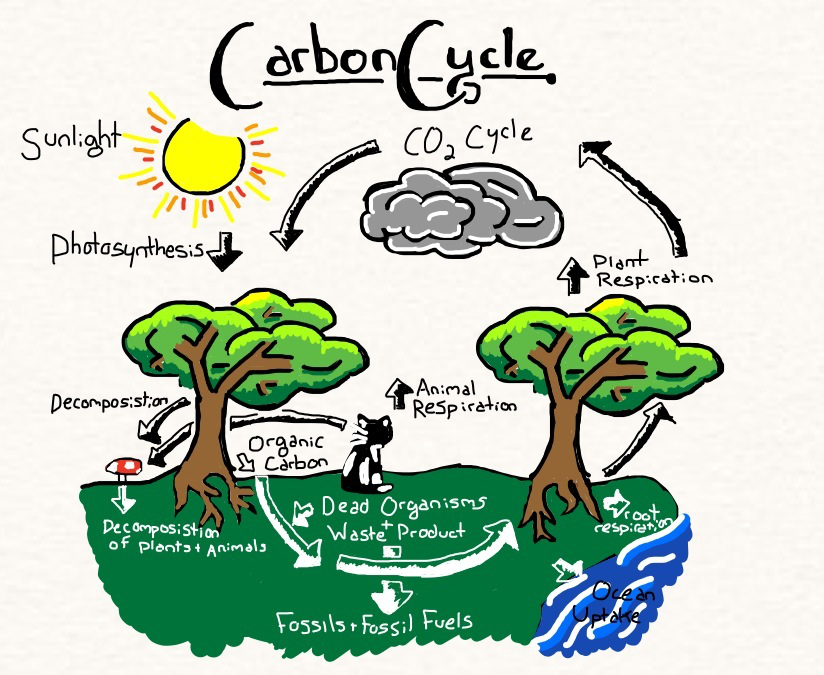
\includegraphics[width=8cm]{carboncycle.jpg}
\caption{carbon cycle \protect\footnotemark}
\end{figure}
\footnotetext{https://www.lingholic.com/wp-content/uploads/2014/06/Carbon-cycle.jpg}  


\subsection{Construction of Fungal Growth Rate Model}
\subsubsection{Brief Introduction of Modeling Process}
% 生长率模型的构建
To explore how fungi are involved in the decomposition of plant material and wood fibers.It is necessary to know more about the biological characteristics of the fungi involved in decomposition——the growth rate of the fungi. \par 

At this point, we should model the growth rate of the fungus first.This step is not unnecessary and will be crucial to our understanding and subsequent modeling.\par 

We took the several steps to model the growth rate of the fungus.\par 

Initially, we wanted to construct a linear model to describe the rate of fungal growth. However, in repeated experiments and comparisons, we found that the traditional linear model was not a good indicator of the growth rate of fungi from a statistical point of view. \par 

However, from the two pictures provided in the question, it can be concluded that there is an exponential relationship between the growth rate of fungus and its moisture tolerance. \par 

When the exponential model is used to describe the relationship between the two, we find that the fitting effect is quite satisfactory.


%The process of establishing the growth rate of fungi is described
% 生长率模型构建的步骤
%\begin{enumerate}[\bfseries 1.]
%    \item Step 1: According to the data provided by the data set, the multiple linear regression model between the growth rate and factors that may be related was constructed. \par 
%    Besides, preliminary screening was conducted to obtain the main variables that affect the growth rate according to the significance level of each independent variable.
%    \item Step 2: The main variables screened out in Step 1 will be verified and interpreted from the biological perspective according to relevant literature. Variables lacking rationality will be excluded. \par 
%    Finally, we will establish the multiple linear regression model of fungi.
%\end{enumerate}\par

\subsubsection{Verify and Interpret Mechanism}

% 验证生长率模型 就是验证耐湿度跟生长率的关系。
We carefully analyzed the data of the relationship between moisture tolerance and decomposition rate given in the question, and found that moisture tolerance had a significant impact on decomposition rate. \par 

In order to prove our point of view, we draw the \textbf{figure \ref{figure:moisture_tolerance_growth_rate}} of moisture tolerance and growth rate, because growth rate will affect decomposition rate.\par

If we find a significant relationship between moisture tolerance and growth rate, we can infer that there is a relationship between moisture tolerance and decomposition rate. \par 

This hypothesis is also consistent with the findings of Daniel S. Maynard et al.\cite{3}, whose analysis revealed a fundamental balance between moisture tolerance and competitiveness, i.e., fungi with broad thermal and water niches exhibit low displacement capacity.\par

The magnitude of this tolerance tradeoff is partly related to the environmental conditions in which the fungi are located, in which the thermal niche traits show the strongest climatic relationship.
\begin{figure}[h]
	\centering
	\begin{tikzpicture}
		\begin{axis}[xlabel = moisture tolerance, ylabel = growth rate]
			\addplot [domain=-1:1, only marks, mark size=0.9pt] table {moisture_tolerance_growth_rate.txt};
			\addplot [domain=-1:1, red] {1.0506*exp(2.3945*x)};
		\end{axis}
	\end{tikzpicture}
	\caption{growth rate curve of moisture tolerance}
	\label{figure:moisture_tolerance_growth_rate}
\end{figure}


%After the significance analysis of multiple regression, it was found that the mycelium density, the optimal temperature, the optimal humidity growth rate, and the precipitation of the wettest month had a significant effect on the growth rate of the fungus.We tried to analyze theoretically why these four variables would have a significant effect on the growth rate of the fungus.\par
%
%1.Mycelium density——The significant effect of mycelium density on the growth rate is not beyond our expectation, and is consistent with our conclusions from previous studies of researchers, and is consistent with Lynne Boddy's hypothesis in the paper that dense mycelium will reduce the decomposition rate of wood.We've also come up with a couple of possible hypotheses.One is the nutrient competition among hyphae——hyphae grow at a fast rate which results in the rapid decrease of some necessary reactive substances in the soil because they are not replenished. It may also be that the production rate of such substances exceeds the consumption rate. Another hypothesis is that the decomposition reaction is exothermic. Due to the high density of mycelia and the fast growth rate, the decomposition reaction is intensified and the exothermic increase which results in the loss of enzyme activity in the soil, and the fragile mycelia die because they cannot absorb enough nutrients.\par
%
%2.The best temperature——Temperature can significantly increase the activities of enzymes in the soil, so that the activities of enzymes reach the maximum at the appropriate temperature.The optimum temperature reflects the adaptation of fungi to the ambient temperature, and when the optimum temperature is in the temperature range where enzymes remain active, it can just accelerate the rate of nutrient absorption by fungi.If the temperature is high enough, the plant can take advantage of the high activity of enzymes in the soil at higher temperatures, gain better survival ability in the harsh natural environment, can maintain competitiveness over a larger range, and accelerate the growth rate of fungi.Using data from Daniel S. Maynard et al., we also plot the relationship between optimal temperature and competitive ranking, and using linear fitting, we find that the higher the optimal temperature, the faster the growth rate, and the higher the ranking of fungi, which is consistent with our initial hypothesis.\par
%
%3.Optimal humidity growth rate——The higher the growth rate, the higher the natural optimum humidity growth rate.The two concepts are very similar.By linear fitting, it is found that there is almost a direct ratio relationship.\par
%
%4.Precipitation in the wettest months--The wettest months are the time of year when the rainfall is the highest, which represents the amount of annual rainfall to some extent. If the wettest months do not meet the humidity and water needed for fungal growth, the growth rate of the fungus will be reduced.Therefore, if the rainfall is higher, the air is more likely to reach the humidity required by the fungus, and it is more likely to maintain the humidity required by the fungus for a longer period of time, thus accelerating the growth rate of the fungus. Our hypothesis results are consistent with the simulation results of our model.

\subsubsection{Simplified to Mathematical Model}
%生长率模型的构建
Set E as the growth rate, a, b, c as constants, and m as moisture tolerance.
\begin{equation}
	\begin{array}{l}
		E=ae^{bM} + C
	\end{array}
\end{equation}

\subsection{Construction of Decomposition Rate Model}
\subsubsection{Brief Introduction of Modeling Process}

%分解率模型与环境与生长速率的关系

In nature, the decomposition process of lignin fiber \cite{} is usually the result of many factors. Therefore, in order to establish the decomposition rate model of wood fiber, we will explore from the perspectives of biological factors and natural environment factors, extract the main influencing factors, and finally get the decomposition model of wood fiber.\par

In the preliminary decomposition rate model of lignin fiber, we adopted the most widely applicable multiple linear regression model.The specific implementation process is as follows: \par

\begin{enumerate}[\bfseries 1.]
	\item According to the data provided by the data set, multiple linear regression analysis was conducted between the decomposition rate of lignin fiber and the factors that might be related to it. \par 
	
	Primary screening was conducted according to the significance level of each independent variable to obtain the major variables with statistical significance.
	
	\item Select the main variables selected in Step 1.According to relevant literature, it is verified and explained in terms of biology and environment.\par 
	
	For the main variables that lack rationality in practical sense, the deletion operation is carried out.The multiple linear regression model of lignin fiber was established preliminarily.
\end{enumerate}\par


%In order to understand how fungi are involved in the decomposition of plant materials and wood fibers, it is necessary to understand the biological characteristics of the fungi involved in the decomposition——the growth rate of the fungi.Consequently, we should model the growth rate of the fungus first.This step is not unnecessary and will be crucial to our understanding and subsequent modeling.\par
%We took the following steps to model the growth rate of the fungus.


%\begin{enumerate}[\bfseries 1.]

%	分解率模型步骤 待补充

%    \item According to the data provided by the data set, the multiple linear regression model between the growth rate and factors that may be related was constructed. Besides, preliminary screening was conducted to obtain the main variables that affect the growth rate according to the significance level of each independent variable.
%    \item The main variables screened out in Step 1 will be verified and interpreted from the biological perspective according to relevant literature. Variables lacking rationality will be excluded. Finally, we will establish the multiple linear regression model of fungi.

%\end{enumerate}

\subsubsection{Verify and Interpret Mechanism}
% 解释四大显著因素 分解率产生影响的原因
Having established and completed the mathematical model of the growth rate, we then proceeded to establish the mathematical model of the decomposition rate.\par

Four variables——growth rate, temperature seasonality, annual temperature range, and rainfall in the wettest months, were found to have significant effects on fungal decomposition rate, i.e., 122 day residual mass, by multiple regression analysis of significance.We have tried to analyze from a theoretical point of view why these four variables have a significant effect on the decomposition rate.\par

1.Growth rate——Fungi need to absorb nutrients from substrates for growth, and the speed of growth reflects the speed of absorption of nutrients by fungi. McGuire and Kristal pointed out in their paper that in classical competition theory\cite{4}, when organisms have similar ecological characteristics, competition for a resource either maintains diversity through niche differentiation or leads to the loss of diversity through the extinction of inferior competitors. Exploitation competition, in which one microbe takes up a resource faster than another, allows a fungus to absorb nutrients more quickly as its growth rate increases.The growth rate was a significant factor in the decomposition rate.\par

2.Temperature seasonality——The seasonality of temperature reflects the temperature difference throughout the year, but if the temperature difference is too large, the growth rate of fungi will be affected. Through the linear model, we can preliminarily understand that when the temperature difference is too large throughout the year, the growth rate will decrease, and we can also conclude that when the growth rate of fungi slows down, the decomposition rate of fungi will be significantly reduced.So temperature seasonality will also be a significant factor in our model.\par

\begin{figure}[h]
	\centering
	\begin{tikzpicture}
		\begin{axis}[xlabel = Temperature seasonality, ylabel = Growth rate]
			\addplot [domain=0:11000, only marks, mark size=0.9pt] table {Temperature_Seasonality_growth_rate.txt};
			\addplot [domain=0:11000, red] {126.06*exp(-0.483*ln(x))};
		\end{axis}
	\end{tikzpicture}
	\caption{growth rate curve of Temperature seasonality}
	\label{figure:Temperature_Seasonality_growth_rate}
\end{figure}

3.Annual temperature range——The annual temperature range, which reflects the extent of annual temperature change, is an important local measure of climate change.The larger the annual temperature range, the greater the likelihood that the temperature will not be within the range of enzyme activity, which will have a significant impact on the final decomposition rate.If the temperature difference is large, it means that in winter, the enzyme will not be able to maintain a high activity, thus affecting the rate of absorption of nutrients by the fungus,reduce growth rate in the \textbf{figure \ref{figure:Temperature_Annual_Range_growth_rate}},and ultimately affecting the size of the decomposition rate.\par

\begin{figure}[h]
	\centering
	\begin{tikzpicture}
		\begin{axis}[xlabel = Temperature annual range, ylabel = Growth rate]
			\addplot [domain=100:450, only marks, mark size=0.9pt] table {Temperature_Annual_Range_growth_rate.txt};
			\addplot [domain=100:450, red] {136.56*exp(-0.751*ln(x))};
		\end{axis}
	\end{tikzpicture}
	\caption{growth rate curve of Temperature annual range}
	\label{figure:Temperature_Annual_Range_growth_rate}
\end{figure}

4.Precipitation of wettest month——The amount of precipitation is an indirect indicator of how wet the air is, and the wettest months tend to represent how much rain falls throughout the year.The figure below reflects the relationship between precipitation and growth rate in the wettest months through linear fitting in the \textbf{figure \ref{figure:Precipitation_of_Wettest_Month_growth_rate}}.The higher the precipitation, the higher the fungal growth rate, so we can infer the relationship between the precipitation in the wettest months and the decomposition rate.\par

\begin{figure}[h]
	\centering
	\begin{tikzpicture}
		\begin{axis}[xlabel = Precipitation of wettest month, ylabel = Growth rate]
			\addplot [domain=100:400, only marks, mark size=0.9pt] table {Precipitation_of_Wettest_Month_growth_rate.txt};
			\addplot [domain=100:400, red] {0.0102*x + 1.8739};
		\end{axis}
	\end{tikzpicture}
	\caption{growth rate curve of precipitation of wettest month}
	\label{figure:Precipitation_of_Wettest_Month_growth_rate}
\end{figure}

\subsubsection{Simplified to Mathematical Model}
\begin{equation}
\begin{cases}
D=\sum\limits_{i=1}^{n}D_i\\
D_i=\alpha_{i1} E_i+\alpha_{i2} T_s+\alpha_{i3}T_R+\alpha_{i4}P_w\\
%E_i=E_i(M_i,T,P)\\
\end{cases}
\end{equation}


%第二问从这里开始

\section{The Interactions Between Different Species of Fungi}

%问题二框架:
%
%第一部分:真菌分类
%为了进一步了解真菌种群间相互作用,我们采用K-means 聚类,系统聚类算法以及肘部法则,根据真菌自身的性状特征进行聚类分析。
%具体流程图如下:

\subsection{Fungi Classification}
In order to further understand the interaction between fungal populations, K-means clustering, systematic clustering algorithm and elbow rule were adopted to conduct cluster analysis according to the characteristics of fungi themselves.\par
The detailed flow chart is as follows (\textbf{figure \ref{figure:flow_chart}}).\par

\begin{figure}[h]
	\centering
	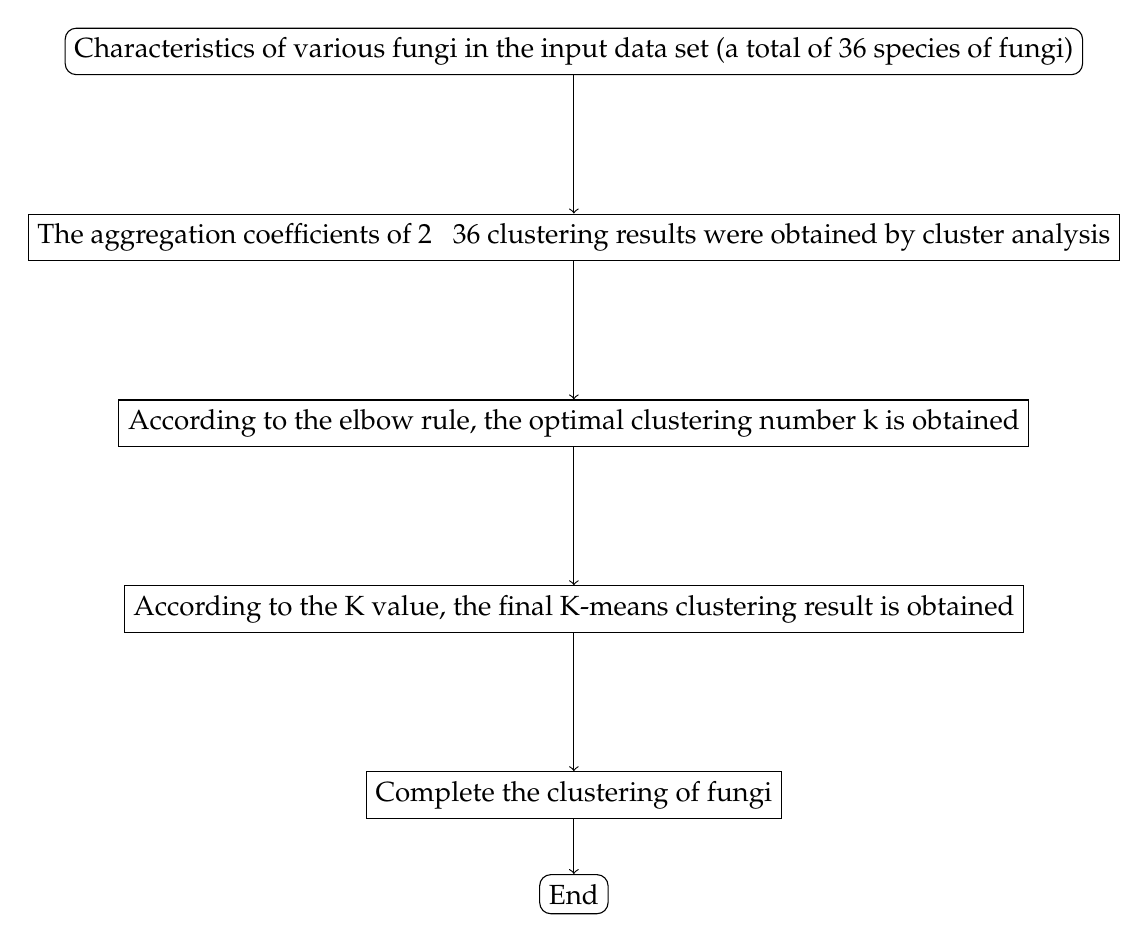
\begin{tikzpicture}[node distance=50pt]
		
		\node[draw, rounded corners]                        (start)   {Characteristics of various fungi in the input data set (a total of 36 species of fungi)};
		\node[draw, below=of start]                         (step 1)  {The aggregation coefficients of 2 ~ 36 clustering results were obtained by cluster analysis};
		\node[draw, below=of step 1]                        (step 2)  {According to the elbow rule, the optimal clustering number k is obtained};
		\node[draw, below=of step 2]                        (step 3)  {According to the K value, the final K-means clustering result is obtained};
		\node[draw, below=of step 3]                        (step 4)  {Complete the clustering of fungi};
		\node[draw, rounded corners, below=20pt of step 4]  (end)     {End};
		
		
%		\node[draw, diamond, aspect=2, below=of step 2]     (choice)  {Choice};
%		\node[draw, right=30pt of choice]                   (step x)  {Step X};
	
	
		\draw[->] (start)  -- (step 1);
		\draw[->] (step 1) -- (step 2);
		\draw[->] (step 2) -- (step 3);
		\draw[->] (step 3) -- (step 4);
		\draw[->] (step 4) -- (end);	
		
		
%		\draw[->] (step x) -- (step x|-step 2) -> (step 2);
%		\draw[->] (step 2) -- (choice);
%		\draw[->] (choice) -- node[left]  {Yes} (end);
%		\draw[->] (choice) -- node[above] {No}  (step x);
	\end{tikzpicture}
	\caption{Flow chart of clustering}
	\label{figure:flow_chart}
\end{figure}



\subsubsection{Assumptions Based on the Above Clustering Results}

%由系统聚类算法得到的谱系图(见群图),
%为了得到最佳聚类数量K,我们对不同聚类数量的聚合系数进行比对,通过肘部法则得到了最终最优的聚类数量是4类(K=4)。这4类真菌的分类情况。(见群图)
%基于上述聚类结果,我们可以做如下假设
The pedigree diagram obtained by the system clustering algorithm(\textbf{figure \ref{figure:Pedigree_diagram}}).\par

\begin{figure}[h] % h为当前位置,!htb为忽略美学标准,htbp为浮动图形
	\centering
	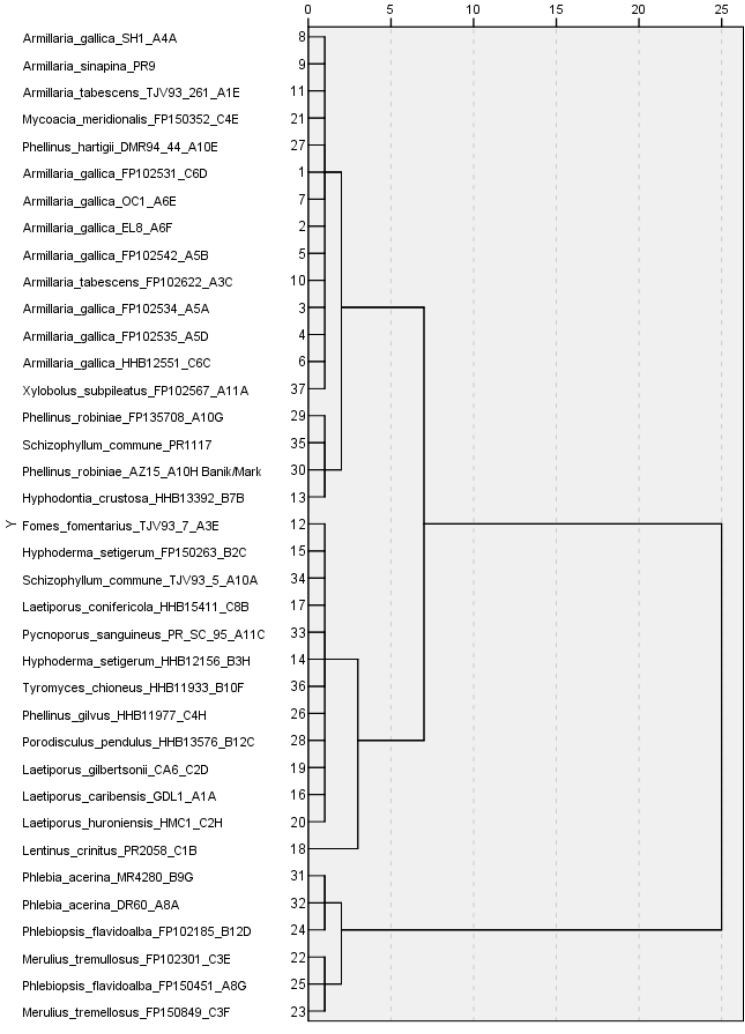
\includegraphics[scale=0.9]{pu-xi-tu.png}
	\caption{Pedigree diagram}
	\label{figure:Pedigree_diagram}
\end{figure}


In order to obtain the optimal number of clustering K,we compared the aggregation coefficients of different cluster numbers, and obtained the final optimal number of clusters by elbow rule is 4 (K=4).The classification of these four types of fungi.
Based on the above clustering results, we can make the following assumptions:\par


\begin{enumerate}[\bfseries 1.]
	%1.	属于同一类别的真菌,既拥有高度相似生物性状的真菌,在木制纤维的分解过程中的作用相似。
	%2.	不同类别的真菌,既拥有较低相似生物性状的真菌,在木制纤维的分解过程中起着不同的作用。
	\item Fungi belonging to the same category, which have highly similar biological traits, play similar roles in the decomposition process of wood fibers.\par
	\item Different types of fungi, including those with relatively low similar biological traits, play different roles in the decomposition of wood fibers.\par
\end{enumerate}\par

\subsubsection{Analysis of Clustering Results}
Through K-means clustering, we finally divided 37 species of fungi given in the data set into three types(\textbf{figure \ref{figure:clustering_results_type}}).\par

\begin{figure}[h]
	\centering
	\begin{tikzpicture}
		\begin{axis}[xlabel = Moisture trade-off, ylabel = Growth rate]
			\addplot [domain=-1:1, only marks, mark size=0.9pt, red] table {clustering_results_type1.txt};
			\addplot [domain=-1:1, only marks, mark size=0.9pt, green] table {clustering_results_type2.txt};
			\addplot [domain=-1:1, only marks, mark size=0.9pt, blue] table {clustering_results_type3.txt};
		\end{axis}
	\end{tikzpicture}
	\caption{K-means clustering results}
	\label{figure:clustering_results_type}
\end{figure}

\begin{figure}[h]
	\centering
	\begin{tikzpicture}
		\begin{axis}[ylabel = J value]
			\addplot+[sharp plot, domain=0:40, mark size=0.9pt, black] table {j_curve.txt};
		\end{axis}
	\end{tikzpicture}
	\caption{J curve}
	\label{figure:J_curve}
\end{figure}

The following is an explanation of the clustering results.\par
The first type (a total of 12 species) tended to have the lowest moisture tolerance and the lowest growth rate of the three types.In addition, the low competitive ability means that this species is at a disadvantage in competing for natural resources, but this type has the widest water niche widths of the three types of fungi.These fungi's ability to better adapt to environmental changes makes up for their lack of competitive species.\par%18
The  second type of fungi (19 species in total) has moderate moisture tolerance and growth rate, and their water niche widths and inter-population competitiveness are also between the first and second type of fungi.\par% 13
The third type (a total of six species) has the strongest moisture tolerance and fastest growth rate, because the first two types compete for natural resources.But that doesn't mean it's any better adapted to its environment.It has the smallest number of species.The narrowest water niche widths mean that these funji are also poor at adapting to environmental changes.\par
In fact, the above conclusions are consistent with the opinion of Daniel S. Maynard et al. in the paper\cite{3}.

%以上是 第一部分聚类

%第二部分:真菌间相互作用的合并
%在上一部分中,我们对真菌进行了具体的分类......
%现在我们从两方面来进行探讨真菌间的相互作用。
%对于同一类别的真菌,由于生物性状的高度相似,同一类别在木制纤维的分解过程中的作用也呈现相似关系。
%因此,为了简化模型和进一步分析,我们采取这样的操作:选取各类别中距离聚类中心最近的真菌作为该类别的代表。由于相似度的影响起着主要作用,故可忽略类别内部的差异。

\subsection{The Merging of Fungal Interactions}
In the previous part, we gave a specific classification of fungi...
Now let's look at the interaction between fungi in two ways.
For fungi of the same class, due to the high similarity of biological characters, the same class also showed similar relationship in the decomposition process of wood fiber.
Therefore, in order to simplify the model and further analysis, we adopted the following operation: the fungi closest to the cluster center in each category were selected as the representative of this category.Since the influence of similarity plays a major role, the differences within categories can be ignored.


%对于不同类别间的真菌,(可引入竞争生态位的概念,麻烦补充相关文献内容)
%不同类别间的真菌,它们的生物性状的相似度较低,一方面在木制纤维的分解过程中承担不同的任务,另一方面它们之间会存在竞争资源的关系,从而直接体现在各自的生长速率受到影响。
%事实上,根据(论文25)所提供的数据集,以及文献中的内容(引用论文25关于ranking的话)......
%我们可对真菌生长速率模型中关于菌丝密度项进行修正,并且考虑到种群的演变。
For fungi between different classes
Fungi of different categories have low similarity in their biological traits. On the one hand, they undertake different tasks in the decomposition process of wood fibers; on the other hand, they compete for resources, which is directly reflected in the influence of their respective growth rates.
In fact, based on the data set provided\cite{3}, we can modify the mycelium density term in the fungal growth rate model and take into account the evolution of the population.

%第三部分:对初步模型的优化
%在上一章节中,我们已经得到了真菌生长率和木质纤维分解率的模型,显然该模型未考虑真菌间的相互作用,离现实模型仍存在偏差。
%在本章节中,我们进行了具体的分析,考虑了种群内部和种群间的相互作用,对初步建立的多元线性回归模型进行推广至广义的的多元线性回归模型。

\subsection{The Optimization of The Preliminary Model}
In the previous chapter, we have obtained the models of fungal growth rate and lignofiber decomposition rate. Obviously, this model does not take into account the interaction between fungi, which is still discrepant from the real model.
In this chapter, we carry out specific analysis, take into account the interaction within and between populations, and extend the preliminarily established multiple linear regression model to the generalized multiple linear regression model.


%可得到最终的优化模型如下
\subsubsection{Simplified to Mathematical Model}

We need to revise the model in the previous chapter because different types of fungi all need to absorb certain organic matter in the wood fiber to maintain their growth, so there is a competitive relationship between them. For simplicity of form, we introduce biomass $C_{xi}$ as one of the variables. Based on the Monod equation in microbial dynamics and the traditional inter-population competition model, the following model is constructed\cite{14}:\par

\begin{equation}
	\begin{cases}
		E_{i} = \frac{\mu_{i}R}{k_{i}+R} \cdot C_{xi} \\
		R=1-D\\
		\frac{\partial C_{xi}}{\partial t} = E_i - \frac{\partial D}{\partial t} \cdot C_{xi}\\
	\end{cases}
	\label{con:you-hua-hou}
\end{equation}

For better illustration, we enumerate only two types of fungi competing, and assume that the natural environment remains unchanged, and consider $C_{xi}$ as a function of time $t$.

The above system of equations is an ordinary differential system. If $\mu_1$>$\mu_2$, in the steady-state solution $\bar{C_{x_2}} = 0$. In fact, $\mu_1$ and $\mu_2$ is actually related to the maximum growth rate $E_{imax}$ in the microbial dynamics, which indicates that the species with the highest growth rate will become the dominant species, and the species with the lowest growth rate will face elimination, which also reflects the natural law of survival of the fittest.

% 添加指数项的理由——请结合figure2说一说

%第二问结束

%第三问开始

\subsection{The Interactions Between the Different Types of Fungi}

In order to analyze the dynamics of the interactions which include both short- and long-term trends, let us might as well start with decomposition rate models contributed by each type of fungi. Because the effect of fungi on the decomposition rate is a direct reflection of the interactions between fungi.\par

Some parameters related to weather or climate can be regarded as constant values over a short period of time, so the degree of decomposition of lignin fibers in which fungi are involved is linearly related to this period of time.In addition, after determining the species of fungus, its moisture tolerance is fixed, so we can obtain:\par

$$
D_i \varpropto E_i
$$


This suggests that the rate of decomposition during this time period depends on the dynamics of the interactions between the fungi.At this time, the dominant factor of interaction among different species of fungi is the competition for resources and space among fungal populations.\par 

At this point, the dynamics of the interactions between fungi can be determined by the equations in the previous chapter.\par
%  (最后填上去) 待填写
Therefore, the decomposition rate contributed by various fungi can be understood as the cumulative effect of fungi and natural factors over time.\par
At the same time, as the content of wood fiber changes, the dynamics of the interactions between fungi will be affected.\par 
Specific relationships can be analyzed through the equations, but it is important to note that natural environmental factors have also played a role.\par

\subsection{Examine the Sensitivity Rapid Fluctuations in the Environment}

In the linear model of decomposition rate, growth rate has maximum weight among the variables. When the natural environmental conditions fluctuate rapidly, only when the fluctuation range is severe enough, the influence of natural environmental factors could be further expanded.

According to the equations \ref{con:you-hua-hou}, when the natural environmental conditions fluctuate rapidly, the derivative value of environmental variables with respect to time changes rapidly, which will also lead to the rapid change of partial derivative value of wood fiber decomposition rate and fungus growth rate with respect to time.

Considering the survival mechanism of fungal population, the fungi with faster growth rate have a narrow niche width, which means that they are less adaptable to the rapid fluctuations in the environment . However, fungi with low growth rate and humidity tolerance can adapt to the changes of natural environment. Therefore, the rapid fluctuation of natural environmental conditions is often accompanied by population succession.






%第三问结束



%第四问开始
\section{Predictions About The Relative Advantages And Disadvantages}
\subsection{Predictions About The Relative Advantages And Disadvantages For Each Species And Combinations of Species}
In the previous section, we have divided the 37 fungal species given in the data set into three broad categories.\par 

The first type of fungi (18 species in total) has low moisture tolerance, low growth rate and high water niche widths.\par 

The second type of fungi (13 species in total) has moderate moisture tolerance and growth rate, and their water niche widths are between the first and second type of fungi.\par 

The third group (a total of six species) has the highest moisture tolerance and fastest growth rate, but the narrowest water niche widths.\par 

To a large extent, growth rate reflects the ability of fungi to compete for natural resources. We made a regression analysis of growth rate and competitiveness ranking, and found that there was a positive correlation between the two. \par 

In the case that the environmental humidity does not exceed the tolerance range of fungi, those with a fast growth rate will undoubtedly occupy more resources, thus establishing advantages, rapid growth and reproduction, while those with a slow growth rate will be in a disadvantaged position.\par 

The moisture tolerance is a combination of many factors, which to some extent reflects the survival ability of fungi, and also reflects the maximum tolerance of fungi to environmental humidity.The more moisture tolerant the fungus is, the more humidity it can live in.When the ambient humidity exceeds the moisture tolerance range, the fungus will die.\par 

The water niche width reflects the ability of fungi to adapt to environmental changes.The higher the width of the water niche is, the less it is affected by the same environmental change, that is, the stronger the resistance is. Fungi with smaller niche widths are more likely to die in the face of short, rapid changes in weather. \par 

Therefore, for the strains with low growth rate and low moisture tolerance, the wider water ecological width makes up for their lack of competitiveness to some extent.\par 

Based on the model established by the second question, we conclude that the presence of one fungus can inhibit the number of other fungi.On the other hand, there is interdependence and cooperation between different strains to complete the decomposition\cite{13}.In the long run, under a relatively constant external environment, through analysis, we can find that the strains with fast growth rate and slow growth rate can often coexist for a long time, because the strains with slow growth rate consume relatively less nutrients in the same time.\par 

However, strains with moderate growth rate have higher requirements for nutrients, but cannot compete with strains with stronger growth rate and moisture tolerance. If the nutrients are squeezed, the biomass of such fungi will be significantly reduced, and the possibility of population decline will be higher.\par 

In regions with complex climate change, the interactions between populations are even more complex. When in a short period of time the weather volatility, has the high growth rate and narrower niche breadth of fungi amount will be affected by severe, at this time the number of fungi have lower growth rate and wider in the short term will rise, when the external environment to stability, and gradually return to the previous ones, according to the competition model described the relationship between the development.\par 

\subsection{The Survival Of Species In Various Environments}
We then consider the survival of colonies in different environments, including arid, semi-arid, temperate, arboreal, and tropical rain forest.
First, ambient temperature and humidity play a direct role in the growth of fungi.Dryness and hygroscopic conditions will affect the growth of fungi that are not suitable for the water niche. \par 

Therefore, we speculate that the fungal diversity will be affected in the drought environment, and the strains with large water niche width will adapt to more climatic environment.Temperate, arboreal climates have favorable temperatures and humidity, which makes it easier for various fungi to survive.Tropical rainforests are more hospitable to fungi that are resistant to moisture and heat.\par 

In addition, seasonal changes in precipitation will produce soil dry-wet alternation, which will promote and inhibit the quantity and activity of soil fungal organisms, and the colonies with large niche width will benefit from it.\par 

On the other hand, carbon and nitrogen are indispensable elements for the growth of fungi, and soil carbon and nitrogen factors are greatly affected by hydrothermal conditions.According to "Effects of Decomposition of Dead Leaves of Typical Plants on Soil Organic Carbon and Nitrogen Transformation and Microbial Diversity in Loess Hilly Region"\cite{12}, "Decomposition of Dead Leaves and Roots of Plants can significantly increase soil organic carbon and nitrate nitrogen contents in 0-5cm and 5-15cm soils".It was found that the increase of soil bacteria and fungi was staged by dead leaves.In the early and middle stages, soil microorganisms are in a process of constant adjustment, so leaf litter can change soil microbial community structure and improve microbial community diversity at the same time.\par 

In the later stage, under the action of litter, the number of fungi increases significantly, which plays a positive role in the survival and reproduction of fungi.In arid and semi-arid regions, vegetation is scarce, so the number of dead leaves which can improve fungal diversity is less than that in temperate and arbor regions.The variety of vegetation species in the tropical rain forest has improved the superior conditions for the growth and reproduction of fungi.\par  

In addition, the influence of different plants on the fungal community is also very different.The paper "Dynamic Characteristics of Wetland Fungal Community Around Onion Leaves" \cite{12}(National Plateau Wetland Research Center, Southwest Forestry University, 2019.2.17) studied the influence of aquatic plants on the structure of wetland fungal community.The results of sampling showed that the Alpha and Beta diversity of the fungal community was low, the community structure was simple, and the obligate attachment relationship of the fungal community on the surface was stable and the similarity was high.\par 

In addition, it should be noted that microorganisms and vegetation may compete for nutrients under certain conditions.In “Changes of Soil Microbial Diversity at Different Altitudes in Wuyi Mountain”\cite{12}. A large number of experiments and detailed analyses were made on the vegetation and fungal community structure at different altitudes.The paper points out that for the survival and reproduction of microorganisms, the temperature rises in spring, the activity of microorganisms increases, and the nutrients accumulated in autumn can be released instantly, which provides rich nutrients for fungi, and the number of fungi increases sharply. \par 

Summer is the peak season for plant growth. Fungi and plants are in nutrient competition, and the nutrients available to bacteria are sharply reduced, resulting in insufficient growth substrates and a sharp decline in the number. In autumn, due to the input of dead leaves and the increase of substrate, the growth of fungi appeared the second exponential growth period.However, as the temperature drops, the growth of the fungus slows down.The lowest temperature in winter, microbial activity is inhibited, fungi in the dead or dormant state, most stop growth and reproduction, so the number of sharp decline.\par 

Therefore, we can infer that the fungal community structure of tropical rain forest is relatively constant due to high temperature and rainy weather throughout the year, and is subject to little seasonal change.\par 


\begin{figure}[h]
	\centering
	\begin{tikzpicture}
		\begin{axis}[xlabel = Time, ylabel = Number of fungi(*$10^{5}$CFU/g drysoil), xticklabels = {,}]
			\draw (10,0) node[below=-5pt]{Apr.};
			\draw (40,0) node[below=-5pt]{Jul.};
			\draw (70,0) node[below=-5pt]{Oct.};
			\draw (100,0) node[below=-5pt]{Jan.};
			\addplot [domain=-1:13, only marks, mark size=0pt]coordinates {(0,-0.5)};
			\addplot [sharp plot,mark size=2pt, mark=square] table {forth-problem/figure1/first.txt};
			\addplot [sharp plot,mark size=2pt, mark=square] table {forth-problem/figure1/second.txt};
			\addplot [sharp plot,mark size=2pt, mark=circle] table {forth-problem/figure1/third.txt};
			\addplot [sharp plot,mark size=2pt, mark=square] table {forth-problem/figure1/forth.txt};
		\end{axis}
	\end{tikzpicture}
	\caption{Seasonal dynamics of fungi in different soil layers}
	\label{figure:Precipitation_of_Wettest_Month_growth_rate}
\end{figure}


\begin{figure}[h]
	\centering
	\begin{tikzpicture}
		\begin{axis}[xlabel = Time, ylabel = Number of fungi(*$10^{5}$CFU/g drysoil), xticklabels = {,}]
			\draw (10,0) node[below=-5pt]{Apr.};
			\draw (40,0) node[below=-5pt]{Jul.};
			\draw (70,0) node[below=-5pt]{Oct.};
			\draw (100,0) node[below=-5pt]{Jan.};
			\addplot [domain=-1:13, only marks, mark size=0pt]coordinates {(0,-0.5)};
			\addplot [sharp plot,mark size=2pt, mark=square] table {forth-problem/figure2/first.txt};
			\addplot [sharp plot,mark size=2pt, mark=square] table {forth-problem/figure2/second.txt};
			\addplot [sharp plot,mark size=2pt, mark=circle] table {forth-problem/figure2/third.txt};
			\addplot [sharp plot,mark size=2pt, mark=square] table {forth-problem/figure2/forth.txt};
		\end{axis}
	\end{tikzpicture}
	\caption{Seasonal dynamics of fungi in different soil layers}
	\label{figure:Precipitation_of_Wettest_Month_growth_rate}
\end{figure}

\begin{figure}[h]
	\centering
	\begin{tikzpicture}
		\begin{axis}[xlabel = Time, ylabel = Number of fungi(*$10^{5}$CFU/g drysoil), xticklabels = {,}]
			\draw (10,0) node[below=-5pt]{Apr.};
			\draw (40,0) node[below=-5pt]{Jul.};
			\draw (70,0) node[below=-5pt]{Oct.};
			\draw (100,0) node[below=-5pt]{Jan.};
			\addplot [domain=-1:13, only marks, mark size=0pt]coordinates {(0,-0.5)};
			\addplot [sharp plot,mark size=2pt, mark=square] table {forth-problem/figure3/first.txt};
			\addplot [sharp plot,mark size=2pt, mark=square] table {forth-problem/figure3/second.txt};
			\addplot [sharp plot,mark size=2pt, mark=circle] table {forth-problem/figure3/third.txt};
			\addplot [sharp plot,mark size=2pt, mark=square] table {forth-problem/figure3/forth.txt};
		\end{axis}
	\end{tikzpicture}
	\caption{Seasonal dynamics of fungi in different soil layers}
	\label{figure:Precipitation_of_Wettest_Month_growth_rate}
\end{figure}

%\clearpage
\begin{center}
	\setlength{\tabcolsep}{0.7mm}{
		\setlength{\tabcolsep}{1.5mm}{
		\begin{longtable}{cccccc}
			\caption{Distribution of microbial quantity in soils at different altitudes in each month}
			\label{tb:notation}\\
			\toprule  % 顶部线
			\makecell*[c]{Types of\\microorganisms} &Time & \makecell*[c]{Evergreen\\ broadleaf \\ forest}   & \makecell*[c]{Coniferous\\ forest}   & \makecell*[c]{Subalpine\\ Coppice}   & \makecell*[c]{Alpine \\ meadow} \\ 
			\midrule  % 中部线
			\multirow{4}*{bacterial} & Apr. &93.83Ba &100.03Bab& 20.37ABa &221.33Aa \\
			~&Jul.&81.20Aab& 111.07Aab &84. 80Aa &132.00Ab\\
			~&Oct.&115.67Aa &118.73Aa &60.33Aa &117.47Abc\\
			~&Jan.&34.19Ab &21.93Ab &47.90Aa &53.23Ac\\ \\

			\multirow{4}*{Fungus}  
			& Apr. & 0.69Aa
			&0.78Aa
			&0.24Ba
			&0.27Ba\\
			~&Jul.&1.08Aa
			&0.23ABa
			&0.23ABa
			&0.07Ba\\
			~&Oct.&0.47Aa
			&0.93Aa
			&0.56Aa
			&0.28Aa\\
			~&Jan.&0.64Aa
			&0.66Aa
			&0.25ABa
			&0.15Ba \\ \\
			
			\multirow{4}*{Actinomycetes}
			&Apr.&2.76Ab
			&2.02Ab
			&1.64Aa
			&1.54Ab\\
			~&Jul.&6.73Aab
			&2.40Cb
			&3.54BCa
			&5.26ABab\\
			~&Oct.&6.21Aab
			&4.20Aab
			&4.49Aa
			&5.06Aab\\
			~&Jan.&10.5Aa
			&6.02Aa
			&3.99Aa
			&8.39Aa\\ \\
			
			\multirow{4}*{\makecell*[c]{Total\\ number of \\ microorganisms}} 
			& Apr. &97.32Aab 
			&102.88Ba
			&122.22ABa
			&223.14Aa \\
			~&Jul.&88.99Aab
			&113.70Aa
			&88.65Aa
			&137.19Ab \\
			~&Oct.&122.50Aa
			&123.97Aa
			&65.36Aa
			&122.72Ab\\
			~&Jan.&45.75Ab
			&28.61Aa
			&52.15Aa
			&61.75Ab \\
			
			\bottomrule  % 底部线
		\end{longtable}}
	}
\end{center}
%%%%%%%%%%%%%%%
%第四问结束
%%%%%%%%%%%%%%%

%第五问开始

\section{Fungal Species Diversity And Ecological Protection}

\subsection{Relationship between fungal species diversity and carbon dioxide}
We may always intuitively believe that the more biodiversity, the better, but it is not. If each kind of fungus is in a different niche, that is, different kinds of fungi are responsible for different steps in the process of decomposition, such a fungal population has a symbiotic relationship. In this case, the better the biodiversity is, the higher the decomposition rate will be.\par 

The research of Chunyan Yang, Douglas A. Schaefer and others provides us with another idea. As we all know, the decomposition of nature will lead to the emission of carbon dioxide, and the annual emission of carbon dioxide is as much as that of fossil fuels. Therefore, if we understand the specific mechanism of biological decomposition, it will provide a powerful means for countries to deal with global warming. It was found that the decomposition rate of the experimental group with high fungal diversity was lower than that of the control group\cite{5,6,7}.\par 

The diversity of fungi will have a negative impact on the decomposition rate. Therefore, increasing the species diversity of fungal community can effectively reduce the carbon dioxide emissions, and it is a meaningful action to reduce the carbon dioxide emissions of biological factors.\par 

\subsection{Model Simulation In Different Environments}

When we use the model constructed by the third question to increase the number of fungal species, the substrate will be completely decomposed in a longer time. This similar result is consistent with the experimental results of many scientists.\par 

We try to change the difference of environmental nutrients, such as adding a variety of nutrients in the model, then the simulation result is that the decomposition rate of high diversity fungal community has a certain degree of upward trend. This further verifies the correctness of our model.\par 

\subsection{Reasonable Explanation And Hypothesis}

Although from the perspective of model results, the higher the species diversity of fungi, the lower the substrate decomposition rate. But we have to try to explain the mechanism behind this.\par 

\begin{enumerate}[\bfseries 1.]
	
	\item This may be due to the pure diversity effect. When the richness and evenness of fungi increase, it may slow down the decomposition rate of substrates, regardless of the species of fungi.\par 
	
	\item Another possible reason is species selection. Species diversity of fungal community may lead to competitive advantage of fungal species with slow decomposition, thus slowing down the decomposition rate of fungal community.\par 
	
	\item Through consulting the data, it was found that the higher the diversity of microorganisms, the higher the decomposition rate of soil organic matter\cite{8,9}. This may be because the organic matter in soil is more than that in wood substrate, and the niche complementarity between microorganisms drives the positive correlation between diversity and organic matter. We can assume that the niche overlap of fungi will lead to limited nutrient competition, which can be observed in many forests\cite{10}. It is this phenomenon that reduces the decomposition rate of substrate.\par 
	
\end{enumerate}\par


%第五问结束

\section{Two-page Article}
\begin{center}
	{\huge The New Research on the Roles Fungi Play in Ecological Systems}
\end{center}


What’s the the problem background and why fungi?\par 
My honourable young readers, as we know ,carbon cycle describes the continuous exchange and movement of carbon on the earth.And in the carbon cycle process, the decomposition of organic material plays important role,which updates and changes the existing form of carbon.In this process ,especially the degradation of plant material and woody fibers involving fungi, is an essential link.\par 
Recently The author of a recent paper which researches on the decomposition wood by fungi has pointed out  the fungal characters that determine the decomposition rate, and figured out the relationships between some characters. Particularly, slow growing fungal strains can survive and grow better in the presence of environmental changes.\par 
In this problem,we only consider two traits of fungi——growth rate and moisture resistance.Our main goal is to model the decomposition of wood fibers on a given land and in the presence of multiple types of fungi that decompose wood fibers in the fixed area.\par 
Thus it’s essential to study the roles fungi play in ecological systems!\par 


What’s our work?\par 
To show you our conclusion better, let's talk about our work first!\par 
Briefly,our work can be generalized into five parts as follows:\par 

\begin{enumerate}[\bfseries 1.]

	\item According to the data provided by the data set, multiple linear regression analysis was conducted between the decomposition rate of lignin fiber and the factors that might be related to it. \par 
	
	\item Firstly,we initially use regression analysis to establish a multiple linear regression model of the decomposition rate of wood fiber .And established a mathematical model of the growth rate.\par 

	\item Secondly,we use K-Means algorithm to incorporate the interactions between different species of fungi which has different traits.Analyse the interactions between different types. Optimize and verify the growth rate model.\par 

	\item Thirdly,we analyse the dynamics of the interactions and examine the sensitivity to rapid fluctuations.\par 

	\item Then,we predict the relative strengths and weaknesses of each species and its possible persistent species combination and apply to five different environments.\par

	\item Finally,we describe how the diversity of fungal communities of a system impacts the overall efficiency of a system with respect to the decomposition of the ground litter.\par 

\end{enumerate}\par



Predict the importance and role of biodiversity in the varying degrees of variability in the local environment.
(For more details,you can read our solutions.)\par 

What’s our new findings and conclusion?\par 
Fungi with a high growth rate and moisture tolerance are more likely to survive when the environment is relatively stable.While when the weather is changeable,fungi with a large water niche width are more competent.We also further discussed the dependence between fungi and the   environment and found out the possible seasonal changes of fungi in different areas.\par 
Our model successfully shows the relationship between fungal species diversity and decomposition rate. When the fungal species diversity is higher, the decomposition rate will also decrease. Because decomposition will emit carbon dioxide, it also indirectly implies the relationship between species diversity and carbon dioxide. It has positive significance for environmental issues related to greenhouse gas emission reduction, and is helpful to optimize the global carbon cycle and co-build a beautiful earth!\par 
Thanks,my honourable young readers!\par 





%\section{Strengths and Weaknesses}
%\subsection{Strengths}
%\begin{itemize}
%    \item First one...
%    \item Second one ...
%\end{itemize}
%
%\subsection{Weaknesses}
%\begin{itemize}
%    \item Only one ...
% \end{itemize}
\clearpage
\begin{thebibliography}{99} 
\addcontentsline{toc}{section}{References}  %引用部分标题("Refenrence")的重命名
\bibitem{1}Elisa T. Lee, Oscar T. Survival Analysis in Public Health Research. \emph{Go. College of Public Health}, 1997(18):105-134.
\bibitem{2}Wikipedia: Proportional hazards model. 2017.11.26. \texttt{\\https://en.wikipedia.org/wiki/Proportional\_{}hazards\_{}model}
\bibitem{3}D. S. Maynard et al., Consistent trade-offs in fungal trait expression across broad
spatial scales. Nat. Microbiol. 4, 846–853 (2019).
\bibitem{4}K. L. McGuire, K. K. Treseder, Microbial communities and their relevance for ecosystem models: Decomposition as a case study. Soil Biol. Biochem. 42, 529–535 (2010).
\bibitem{5}10 Toljander, Y. K., Lindahl, B. D., Holmer, L. \& Högberg, N. O. S. Environmental fluctuations facilitate species co-existence and increase decomposition in communities of wood decay fungi. Oecologia 148, 625–631, doi: 10.1007/s00442-006-0406-3 (2006).
\bibitem{6}Fukami, T. et al. Assembly history dictates ecosystem functioning: evidence from wood decomposer communities. Ecol. Lett. 13, 675–684, doi: 10.1111/j.1461-0248.2010.01465.x (2010).
\bibitem{7}Lindner, D. L. et al. Initial fungal colonizer affects mass loss and fungal community development in Picea abies logs 6 yr after inoculation. Fungal Ecol. 4, 449–460, doi: 10.1016/j.funeco.2011.07.001 (2011).
\bibitem{8}31Nielsen, U. N., Ayres, E., Wall, D. H. \& Bardgett, R. D. Soil biodiversity and carbon cycling: a review and synthesis of studies examining diversity–function relationships. Eur. J. Soil Sci. 62, 105–116, doi: 10.1111/j.1365-2389.2010.01314.x (2011).
\bibitem{9}32Baumann, K. et al. Soil microbial diversity affects soil organic matter decomposition in a silty grassland soil. Biogeochemistry 114, 201–212, doi: 10.1007/s10533-012-9800-6 (2013).
\bibitem{10}Woodward, S. \& Boddy, L. Interactions between saprotrophic fungi in Ecology of Saprotrophic Basidiomycetes (eds. Boddy, L., Frankland, J. C. \& van West, P. ) 124–139 (Elsevier, 2008).
\bibitem{11}Chi Y J, Liu Z H, Bao F C. Populations and communities of microorganisms growing on wood and their succession regulatioms[J]. Journal of Fungal Biology, 2004, 2: 51-57.
\bibitem{12}Jin Yuhua. Variation characteristics of soil microbial diversity at different altitudes in Wuyishan [D]. Nanjing Forestry University, 2012.
\bibitem{13}Feng Le. Coupling relationship between filamentous fungi and ectomycorrhizal fungi on decomposition of Korean pine litter [D]. Heilongjiang University, 2011.
\bibitem{14}Zang Rongchun. Xia Fengyi. Microbial kinetic model [M]. Beijing: Chemical Industry Press, modern biotechnology and medical science and Technology Publishing Center, 2003.
\end{thebibliography}


% ==============以下为附录内容,如您的论文中不需要程序附录请自行删除====================

%\clearpage
%\begin{subappendices}						% 附录环境
%\section*{Apendix: The source codes}		% 附录标题可以自行修改
%\addcontentsline{toc}{section}{Appendix}  	% 将附录内容加入到目录中
%
%This MATLAB program is used to calculate the value of variable $a$.
%\begin{lstlisting}[language=Matlab, caption=\texttt{temp.m}]
%a = 0;
%for i = 1:5
%	a = a + 1;
%end
%\end{lstlisting}
%
%This LINGO program is used to search the optimize solution of 0-1 problem.
%\begin{lstlisting}[language=Lingo, caption=\texttt{temp.lg4}]
%model:
%sets:
%WP/1..12/: M, W, X;
%endsets
%data:
%M = 2 5 18 3 2 5 10 4 11 7 14 6;
%W = 5 10 13 4 3 11 13 10 8 16 7 4;
%enddata
%max = @sum(WP:W*X);
%@sum(WP: M * X)<=46;
%@for(WP: @bin(X));
%end
%\end{lstlisting}
%
%\end{subappendices}

% =================================================================================



\end{document}